\documentclass[10pt,a4paper]{article}
\usepackage[paper=a4paper, hmargin=1.5cm, bottom=1.5cm, top=3cm]{geometry}

\usepackage[utf8x]{inputenc}
\usepackage[spanish]{babel}

\usepackage{mathtools}
\usepackage{amsmath}
\usepackage{amsfonts}
\usepackage{amssymb}

\usepackage{xcolor}
\usepackage{listingsutf8}
\usepackage{booktabs}
\usepackage{hyperref}
\usepackage{multirow}

\usepackage{caption}

\usepackage{subcaption}
\usepackage{algorithm}
\usepackage[noend]{algpseudocode}

\usepackage{graphicx}
\usepackage{tikz}
\usepackage{relsize}
\usepackage{epstopdf}


\DeclarePairedDelimiter{\ceil}{\lceil}{\rceil}

% set the default code style
\lstset{
    frame=tb, % draw a frame at the top and bottom of the code block
    tabsize=4, % tab space width
    showstringspaces=false, % don't mark spaces in strings
    numbers=left, % display line numbers on the left
    commentstyle=\color{green}, % comment color
    keywordstyle=\color{blue}, % keyword color
    stringstyle=\color{red} % string color
}

% mathy stuff
\newtheorem{theorem}{Theorem}[section]
\newtheorem{lemma}[theorem]{Lemma}
\newtheorem{proposition}[theorem]{Proposición}
\newtheorem{corollary}[theorem]{Corollary}

\newenvironment{proof}[1][Demostración]{\begin{trivlist}
\item[\hskip \labelsep {\bfseries #1}]}{\end{trivlist}}
\newenvironment{definition}[1][Definición]{\begin{trivlist}
\item[\hskip \labelsep {\bfseries #1}]}{\end{trivlist}}
\newenvironment{example}[1][Example]{\begin{trivlist}
\item[\hskip \labelsep {\bfseries #1}]}{\end{trivlist}}
\newenvironment{remark}[1][Remark]{\begin{trivlist}
\item[\hskip \labelsep {\bfseries #1}]}{\end{trivlist}}

\newcommand{\qed}{\nobreak \ifvmode \relax \else
      \ifdim\lastskip<1.5em \hskip-\lastskip
      \hskip1.5em plus0em minus0.5em \fi \nobreak
      \vrule height0.75em width0.5em depth0.25em\fi}

\title{Teoría de las Comunicaciones \\ TP1}

\newcommand{\order}[1]{$\mathcal{O}(#1)$}
\newcommand{\quotes}[1]{``#1''}
\newtheorem{definicion}{Definición}

\begin{document}

%% cover page

\maketitle

\bigskip

\begin{table}[h]
\centering
\begin{tabular}{|l l l|}
\hline
Integrante       & \multicolumn{1}{c}{LU}     & Correo electrónico        \\ \hline
Sosa Juan Cruz & \multicolumn{1}{c}{733/12} & nirvguy@gmail.com \\ 
Lucas Tavolaro Ortiz & 322/12                      & tavo92@gmail.com \\
Mauro Cherubini & 835/13                      & cheru.mf@gmail.com \\ \hline
\end{tabular}
\end{table}

\vfill

\begin{center}
\textbf{Reservado para la cátedra}
\end{center}
\begin{table}[h]
\centering
\begin{tabular}{|l|l|l|}
\hline
Instancia       & Docente & Nota \\ \hline
Primera entrega &         &      \\ \hline
Segunda entrega &         &      \\ \hline
\end{tabular}
\end{table}

\newpage
\tableofcontents
\newpage

% end cover page

\section{Introducción}



\section{Metodologia}
\subsection{Sniffer con Scapy}

Para el an\'alisis de las distintintas redes, realizamos un sniffer utilizando la libreria Scapy en Python 3. La misma utiliza las funciones definidas para poder observar los paquetes que llegan y cada paquete lo procesamos con la fuente que tenemos. Adem\'as, agregamos distintas funcionalidades utiles, como guardar la informaci\'on en formato .pcap para luego poder procesarlo y realizar graficos para visualizar de una mejor manera la informaci\'on.

\subsection{Fuentes de informacion usadas}

Para el presente TP modelamos dos fuentes que puedan generarnos la informaci\'on que queremos analizar. En \textit{fuente.py} definimos una clase que nos sirva para poder modelar las distintas fuentes que necesitamos, adem\'as de poder tener m\'etodos que nos den informaci\'on valiosa como la entrop\'ia y las probabilidades e informaci\'on de cada uno de los simbolos. En \textit{analyse-data.py} definimos dos funciones que se encargan de agregar los simbolos para cada una de las fuentes, en base a los paquetes que se reciben. Analizaremos en detalle este proceso viendo cada una de las fuentes a continuaci\'on.

\subsubsection{Fuente unicast-multicast}

Como dice el nombre, esta fuente nos servir\'a para poder comparar los paquetes unicast contra los multicast. Para esto, observamos la MAC de destino de cada paquete. Si sucede que la MAC de destino es \texttt{ff:ff:ff:ff:ff:ff} nos indica que su destino son todos los nodos del dominio de broadcast, por lo tanto se trata de una direccion multicast. Caso contrario, es decir que el paquete tenga una MAC distinta a antes mencionada, significa que esta dirigido a un \'unico dispositivo y por lo tanto es unicast.

En \textit{analyse-data.py} definimos la funci\'on \textit{analize\_uni\_multi\_cast} que realiza lo que ya describimos tomando como entrada un paquete, y luego en base a su destino genera el simbolo correspondiente, que será unicast o multicast segun corresponda.


\subsubsection{Fuente ARP}

En esta fuente solo nos interesar\'an los paquetes ARP para poder analizar que sucede con ellos. Por lo tanto, todos los paquetes que no sean ARP no generar\'an ning\'un simbolo en esta fuente. Una vez realizado este filtro, generaremos un simbolo de acuerdo al destino que tenga el paquete.

En \textit{analyse-data.py} definimos la funci\'on \textit{analize\_arp} que realiza lo mencionado. Notemos que adem\'as esta funci\'on es utilizada para otro proposito que es el de generar el grafo dirigido de topolog\'ia de la red agregando un eje entre el nodo que representa el dispositivo que envi\'o el paquete y el nodo que representa el que recibi\'o el paquete. Adem\'s decidimos etiquetar con su direcci\'n MAC al nodo que representa los mensajes del tipo brodcast.


\section{Resultados}
En esta secci\'on, presentaremos los resultados obtenidos en los experimentos
utilizando lo definido en la secci\'on de desarrollo.

Se buscaron analizar en cada fuente tres tipos de redes segun su escala, es
decir redes pequeña, mediana y gran escala. Estas redes fueron
una hogareña, de unas oficinas, de un laboratorio de una Universidad.

En cada captura se almaceno todo los paquetes que se transmitieron por la red
con el sniffer desarollado como se menciono previamente. Luego analizados
automaticamente por el otro programa `analy\_data` para producir los graficos
que se presentan a continuación.

\subsection{Nodos distinguidos}

En cada experimento se analizaron las dos fuentes de información y se definió
un criterio para distinguir un nodo de cada red. Este criterio consta en que
será distinguido el símbolo con mas probabilidad de ocurrir o equivalentemente
el símbolo que tenga menor información.

Para la fuente $S_2$ una de las hipótesis es que estos nodos "distinguidos" son
nodos especiales como routers, access points, etc. dado que estos participan
en la mayor parte de las comunicaciones con la red como con el exterior.
Por lo cual esto nos daría un método (no 100\% confiable debido a casos
atípicos) de determinar los router en una red.

Otra de las hipótesis que se presenta es que una red \textit{cableada} será
mas "compresible" que una \textit{wireless}. Para esto se mostraron el
cociente de la $\frac{H(S)}{H_{MAX}(S)}$ como se desarrollo en TODO: CITA
y se los comparo entre el mismo tipo de fuente de los distintos experimentos.

\subsection{Descripción de los Gráficos}

En cada experimentación se generaron tres tipos de resultados/gráficos.

\begin{itemize}
	\item Un gráfico que muestra una representación tipo torta de la fuente,
	esto es, la probabilidad de ocurrencia de cada símbolo.  \item Un gráfico
	tipo histograma que muestra para cada símbolo la información de este. Este
	gráfico cuenta además con una barra horizontal que muestra donde se sitúa
	la Entropía de la fuente (en color naranja) y otra barra similar que
	muestra donde se sitúa la Entropía máxima que podría tener la fuente.
	\item Un gráfico con la topología de los mensajes de la red. Donde los
	nodos son \textbf{MAC} address y las aristas representan un paquete de un
	nodo a otro
\end{itemize}

\subsection{Red hogareña}

En este caso se analizó una red de pequeña escala con 2 notebooks encendidas,
2 celulares y un router.

\subsubsection{Fuente Unicast-Multicast}

 Lo siguiente corresponde a la experimentación realizada para la fuente
 Unicast-Multicast en una red WiFi domestica.
 
\begin{figure}[hp!]
	\begin{minipage}[b]{0.9\linewidth}
		\subfloat[Probabilidades de los simbolos de la fuente $S_1$ para la red de hogareña]{
		 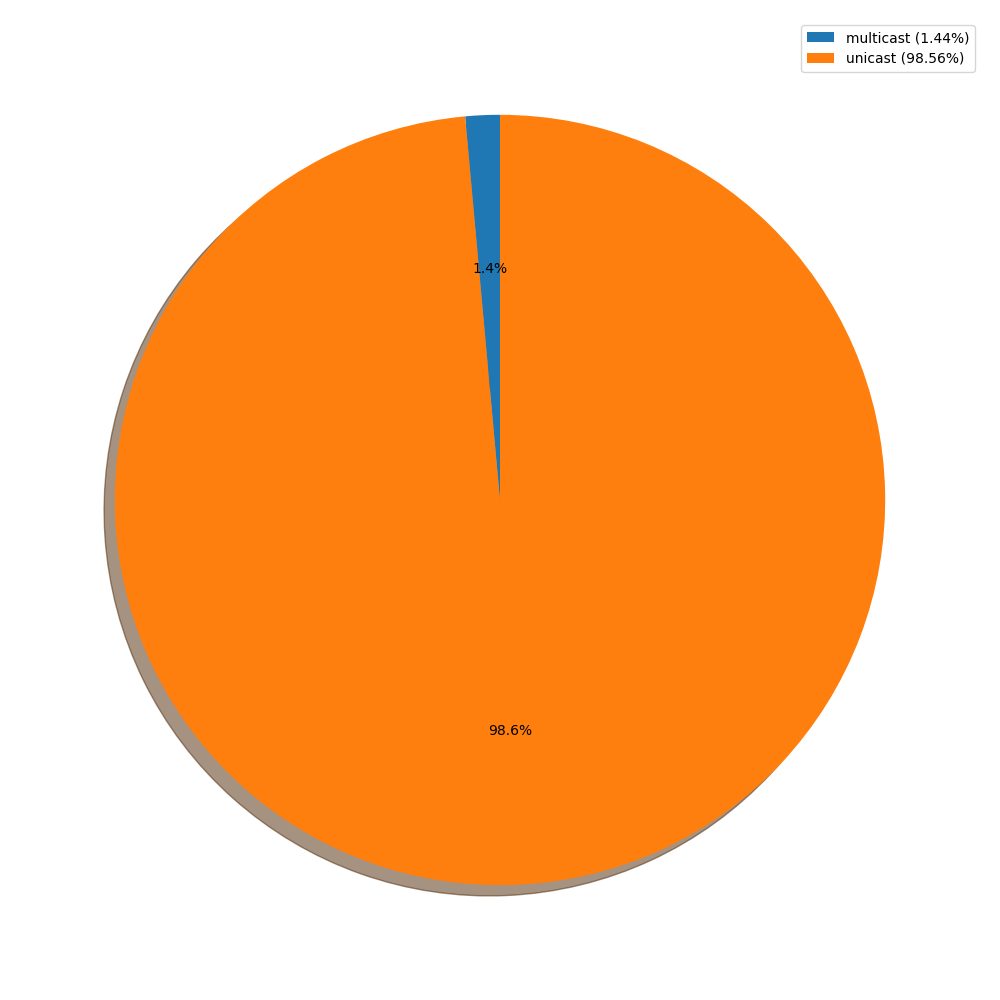
\includegraphics[width=0.45\linewidth]{../plots/mauro_s1_probabilidades.png}
		}
		\subfloat[Información de los simbolos de la fuente $S_1$ para la red de hogareña]{
		 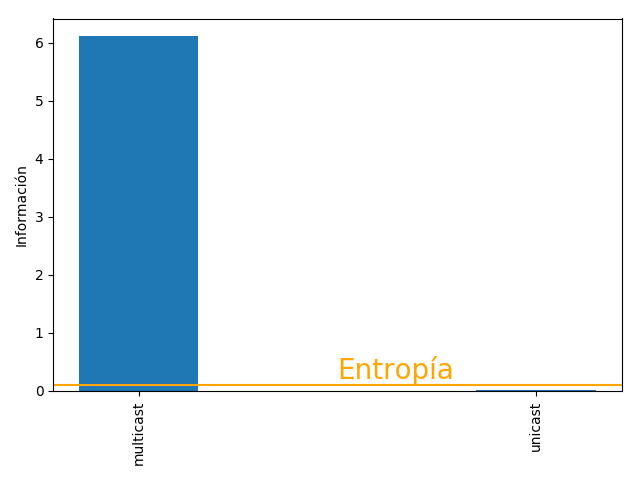
\includegraphics[width=0.55\linewidth]{../plots/mauro_s1_informacion.png}
		}
	\end{minipage}
\end{figure}

Como podemos ver los resultados obtenidos muestran una alta concentración de
paquetes \textit{multicast} por sobre los \textit{unicast}. En consecuencia la
entropía cae abruptamente, ya que como explicamos ésta se maximiza cuando la
distribución de las probabilidades de cada símbolo es equitativa, y baja a
medida que nos alejamos de ello. Nuestra primera impresión era que los
paquetes \textit{unicast} iban a predominar en la captura, sin embargo esto no
sucedió. Es posible que esto se deba a que la placa de red del dispositivo en
el cual se tomó la muestra no hayan entrado en modo promiscuo, en consecuencia
el \textit{sniffer} solo llego a capturar los paquetes cuyo destino era dicho
dispositivo (y no todos los \textit{unicast} transmitidos en la red). Por el
contrario los \textit{multicast} enviados por cualquier dispositivo de la red
se pudieron seguir escuchando sin ningún tipo de censura.

\clearpage
\subsubsection{Fuente ARP}

\begin{figure}[hp!]
	\begin{minipage}[b]{0.9\linewidth}
		\subfloat[Probabilidades de los simbolos de la fuente $S_2$ para la red de hogareña]{
		 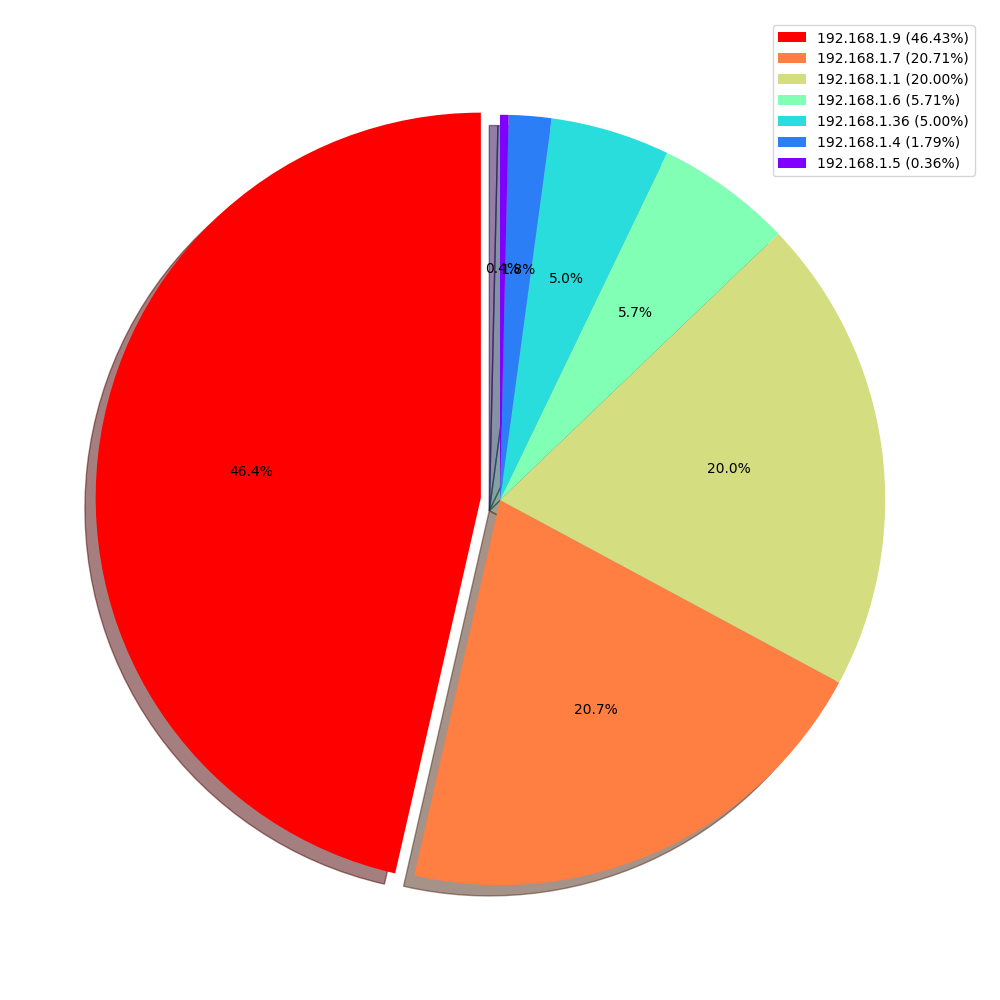
\includegraphics[width=0.45\linewidth]{../plots/mauro_s2_probabilidades.png}
		}
		\subfloat[Información de los simbolos de la fuente $S_2$ para la red de hogareña]{
		 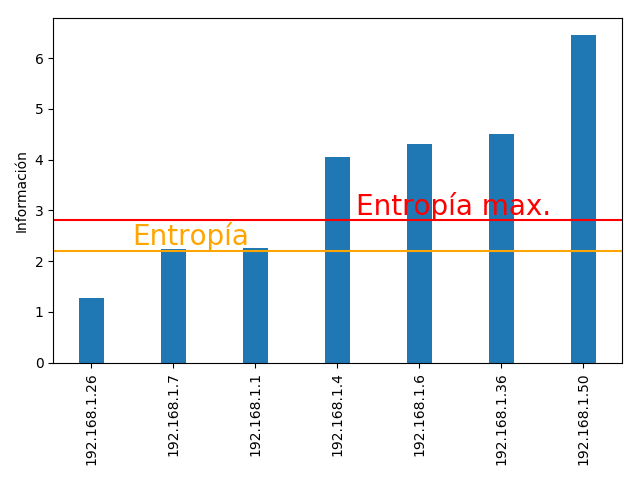
\includegraphics[width=0.55\linewidth]{../plots/mauro_s2_informacion.png}
		}
	\end{minipage}
\end{figure}

Este experimento lamentablemente no dio como esperabamos. La IP 192.168.1.9, se corresponde
a la notebook en la cual se corrio este experimento y no al router. La misma concentro aproximadamente
la mitad de los paquetes ARP de esta red y alcanza 1 de informacion.

\subsubsection{Topolog\'ia de la Red}
\begin{figure}[hp!]
	\begin{center}
	 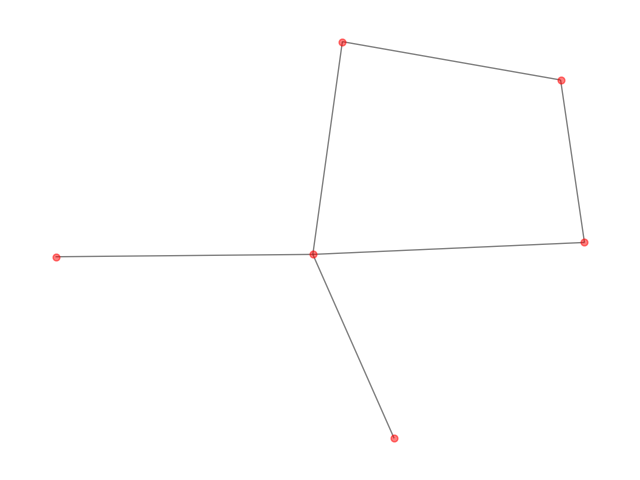
\includegraphics[scale=0.6]{../plots/mauro_s2_topologia.png}
	\end{center}
\end{figure}

Tiene una topolog\'ia estrella como es com\'un en una red domestica. El nodo de mas a la izquierda y
arriba tiene la rareza de que nunca envio un who has, pero si respondio is at a dos nodos de la red.

\subsection{\emph{Red de Oficinas}}

En esta caso se analizo una red cableada de mediana escala, que consta de 6
oficinas con varias computadoras de escritorio (Desktop) totalizando una
cantidad de 29 estaciones. Además en cada oficina se encuentra un switch que
conecta todas las PCs de esta. La captura que se tomó fue de una hora para
poder obtener estadísticamente suficiente precision en las medidas y que estas
no sean alteradas por posibles `outliers`.

\clearpage

\subsubsection{Fuente Unicast-Multicast}

\begin{figure}[hp!]
	\begin{minipage}[b]{0.9\linewidth}
		\subfloat[Probabilidades de los simbolos de la fuente $S_1$ para la red de oficinas]{
		 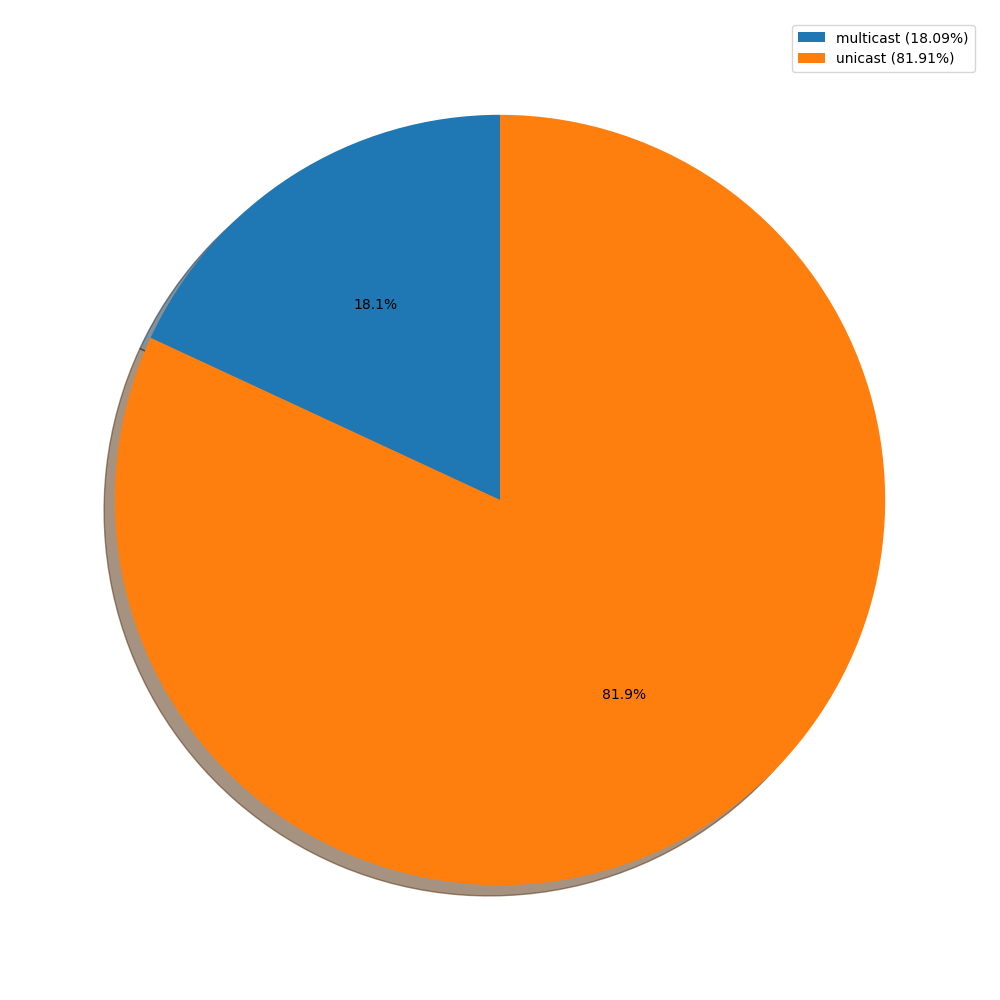
\includegraphics[width=0.45\linewidth]{../plots/trabajo_s1_probabilidades.png}
		}
		\subfloat[Información de los simbolos de la fuente $S_1$ para la red de oficinas]{
		 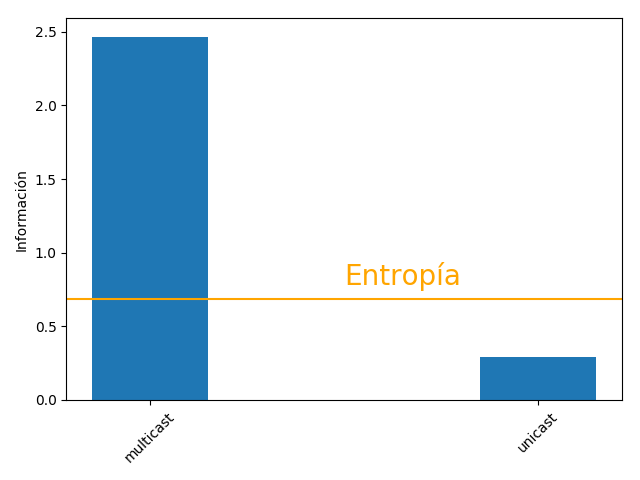
\includegraphics[width=0.55\linewidth]{../plots/trabajo_s1_informacion.png}
		}
	\end{minipage}
\end{figure}


Como se puede observar en ambos gráficos el el símbolo destacado es el
\textbf{unicast}, ya que este tiene mayor probabilidad y menor cantidad de
información. Esto nos dice que aproximadamente sobre el cable el $81.91\%$ los
paquetes fue unicast.  El sentido de esto puede deberse a que los únicos
protocolos que usan el tipo de mensajes broadcast son protocolos de control y
representan una pequeña proporción del trafico total de la red.

\subsubsection{Fuente ARP}

\begin{figure}[hp!]
	\begin{minipage}[b]{0.9\linewidth}
		\subfloat[Probabilidades de los simbolos de la fuente $S_2$ para la red de oficinas]{
		 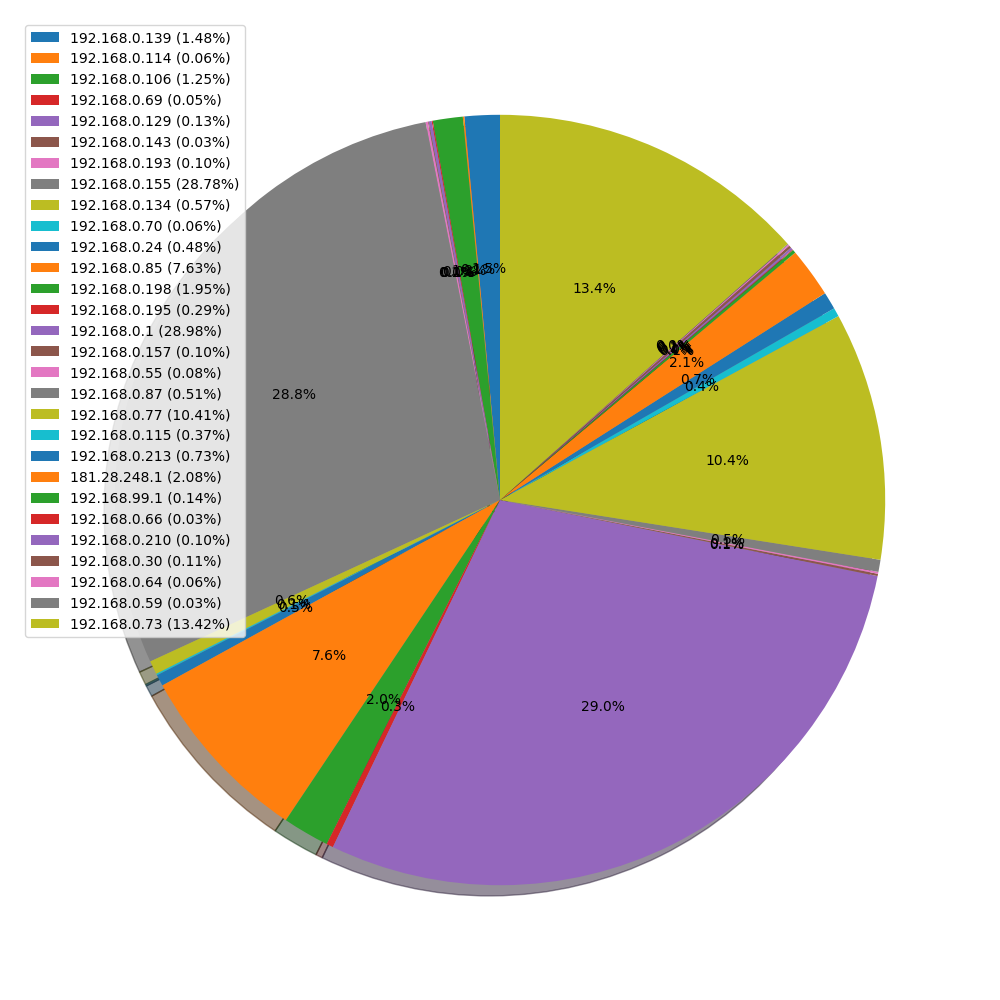
\includegraphics[width=0.45\linewidth]{../plots/trabajo_s2_probabilidades.png}
		}
		\subfloat[Información de los simbolos de la fuente $S_2$ para la red de oficinas]{
		 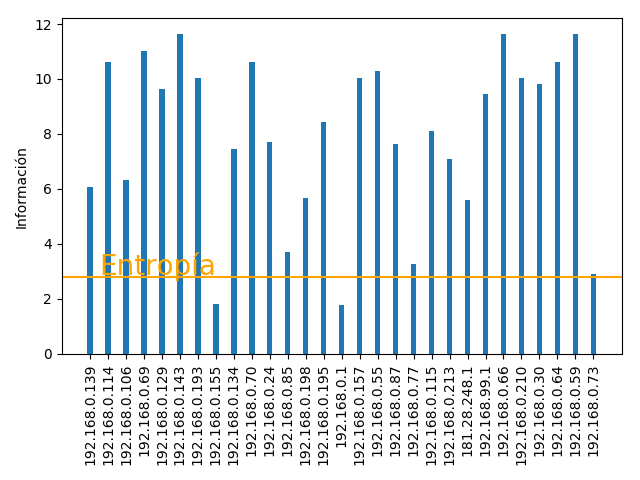
\includegraphics[width=0.55\linewidth]{../plots/trabajo_s2_informacion.png}
		}
	\end{minipage}
\end{figure}

En estos gráficos se puede ver que efectivamente el nodo \textbf{192.168.0.1}
es el destacado. Por previo conocimiento de la red se sabe que este
es el router lo cual refuerza nuestra hipótesis sobre los nodos destacados.
También se observa que la entropía alcanzada es de $2.77$ cuando la máxima
es $4.85$ y por tanto $\eta_{C} = 0.41$

\clearpage
\subsubsection{Topolog\'ia de la Red}
\begin{figure}[hp!]
	\begin{center}
	 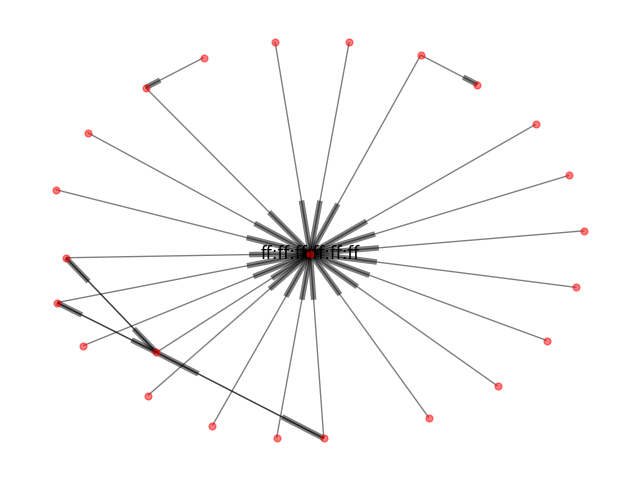
\includegraphics[scale=0.6]{../plots/trabajo_s2_topologia.png}
	\end{center}
\end{figure}

Se puede observar que la topología de mensajes arp es de tipo estrella
y que el grafo es conexo. El nodo del centro resulta ser la MAC $ff:ff:ff:ff:ff:ff$
es decir los mensajes broadcast. Se puede ver que hay pocos nodos que le hayan
enviado un paquete arp a otro que no sea el broadcast. Esto se debe
a que al estar detrás de un switch, los mensajes unicast de respuesta (\textit{is-at})
no son forwardeados a la interfaz de la maquina que realiza la captura aun estando en modo promiscuo
.En cambio cuando se trate de un mensaje unicast que responde el mismo dispositivo que
realiza la captura este si es registrado. Aun asi se filtran mensajes unicast de pc's a otras pc's. Esto como
se dijo puede deberse a switchs que no aprendieron bien la tabla de forwardeo.

\subsection{Red de Laboratorios del DC}

Este experimento fue realizado en una red de gran escala a las 16:00hs durante media hora en los Laboratorios del DC.
Se utilizo la red wifi con el nombre Laboratorios DC.

\subsubsection{Fuente Unicast-Multicast}

\begin{figure}[hp!]
	\begin{minipage}[b]{0.9\linewidth}
		\subfloat[Probabilidades de los simbolos de la fuente $S_1$ para la red de laboratorios]{
		 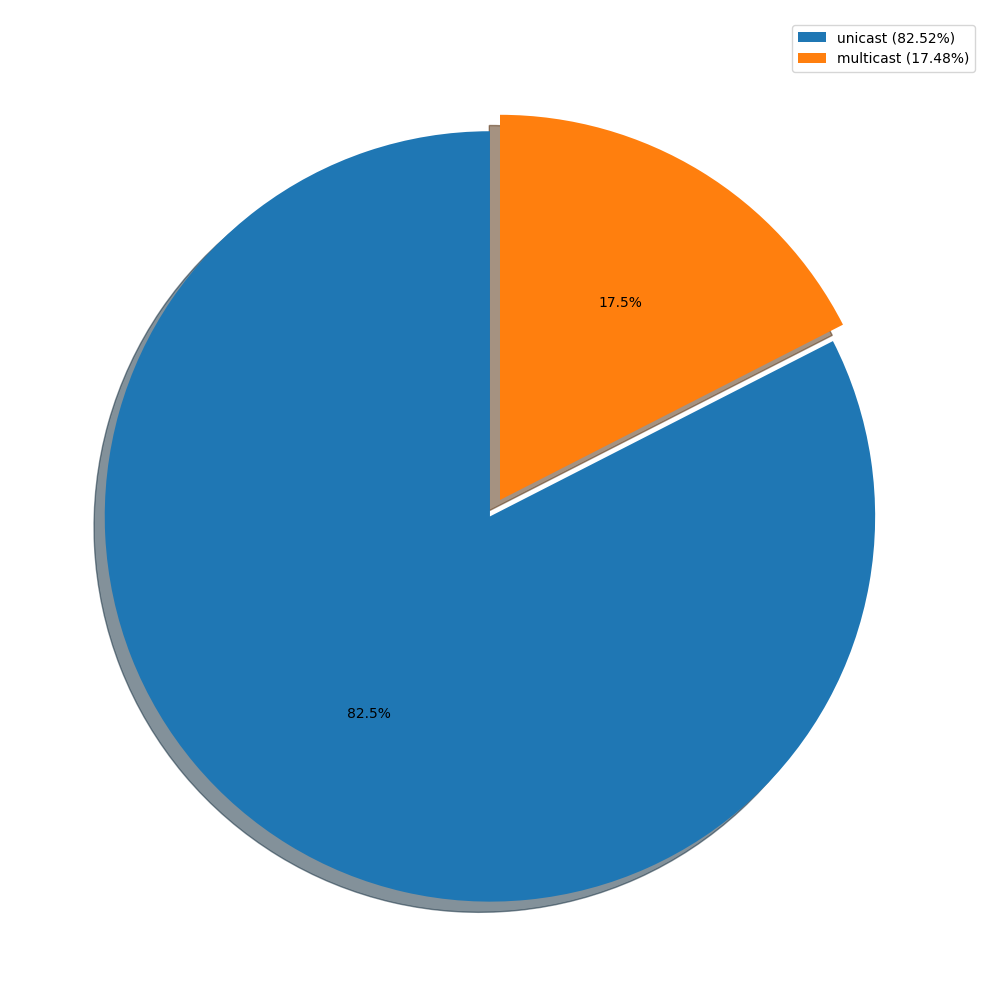
\includegraphics[width=0.45\linewidth]{../plots/labos_s1_probabilidades.png}
		}
		\subfloat[Información de los simbolos de la fuente $S_1$ para la red de laboratorios]{
		 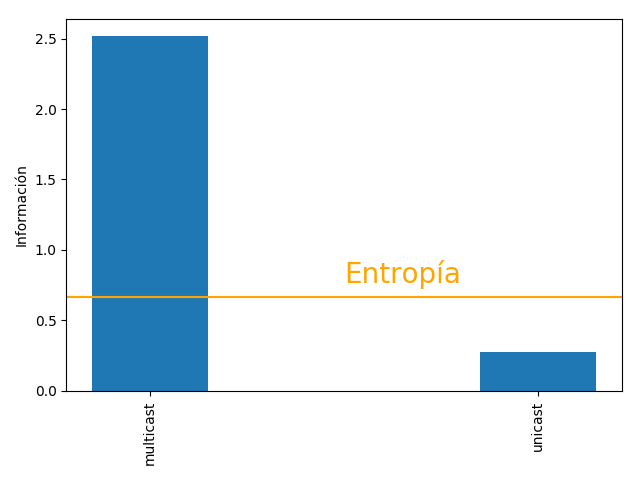
\includegraphics[width=0.55\linewidth]{../plots/labos_s1_informacion.png}
		}
	\end{minipage}
\end{figure}

Como se dijo anteriormente en el caso de la Red de Oficinas, se ve que la mayor\'ia
de los paquetes son unicast porque los paquetes broadcast son usados generalmente
por los protocolos de control. Ademas, la probabilidad de unicast fue de 0.82, la
informacion de 0.27 y la entropia de la fuente de 0.66.

\subsubsection{Fuente ARP}

\begin{figure}[hp!]
	\begin{minipage}[b]{0.9\linewidth}
		\subfloat[Probabilidades de los simbolos de la fuente $S_2$ para la red de laboratorios]{
		 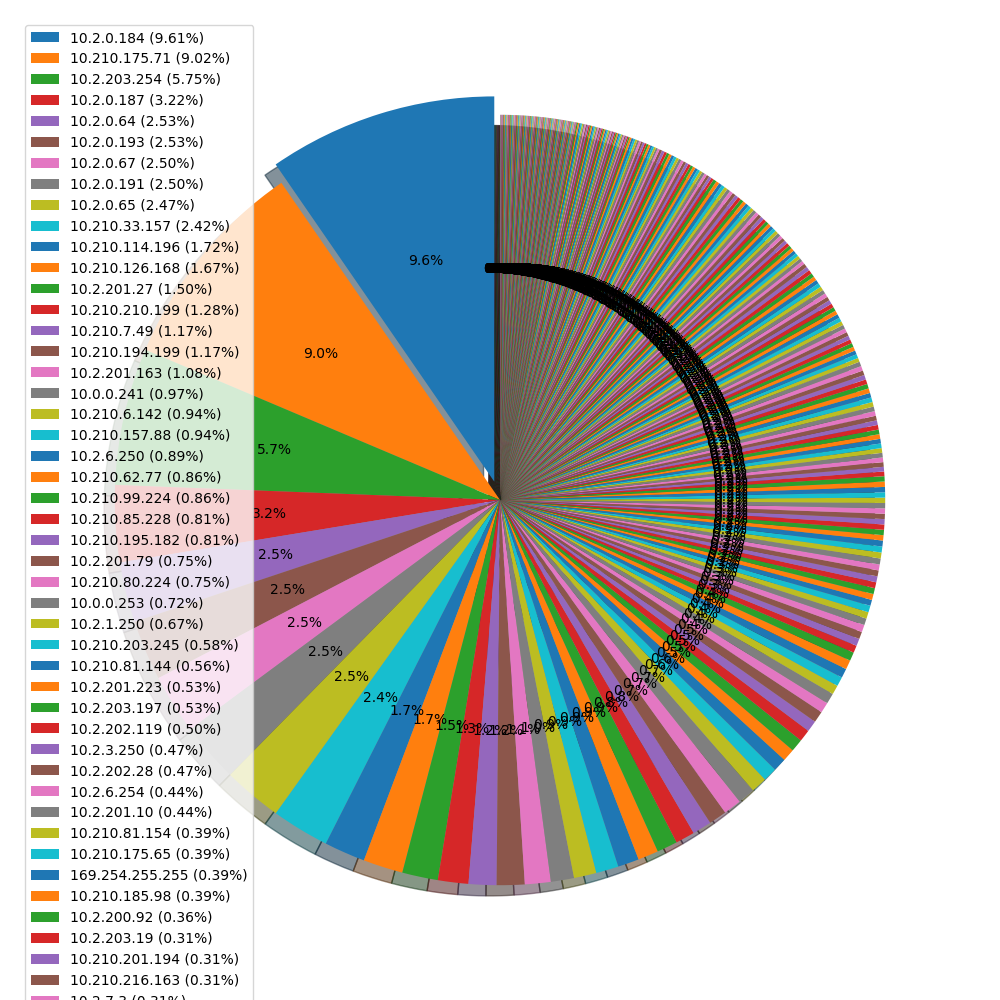
\includegraphics[width=0.45\linewidth]{../plots/labos_s2_probabilidades.png}
		}
		\subfloat[Información de los simbolos de la fuente $S_2$ para la red de laboratorios]{
		 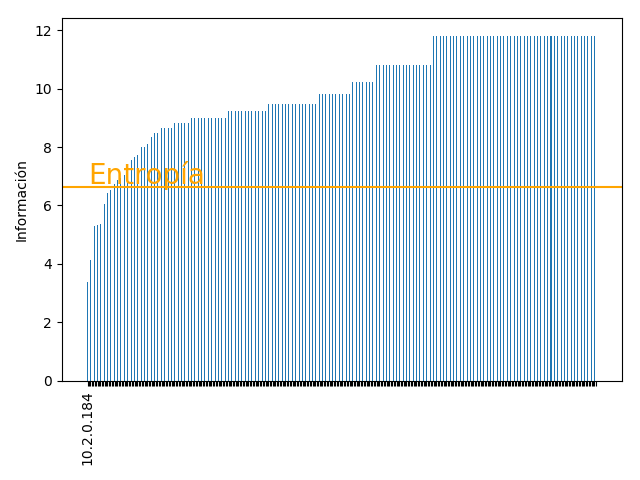
\includegraphics[width=0.55\linewidth]{../plots/labos_s2_informacion.png}
		}
	\end{minipage}
\end{figure}

Podemos observar que en este caso el nodo destacado es de la IP 10.2.0.184 con casi el 10%.
Averiguamos a que dispositivo corresponde y es la impresora, lo que nos hace pensar que
por el horario se estaba usando mucho para imprimir, aunque tambien podria ser
que su tabla ARP tiene una cache con poco tiempo de vida para cada elemento.

En cuanto a la entropia, vemos que es de 6.619, el maximo de 8.484 y la comprensibilidad es
de 0.220.

\subsubsection{Topolog\'ia de la Red}

\begin{figure}[hp!]
	\begin{center}
	 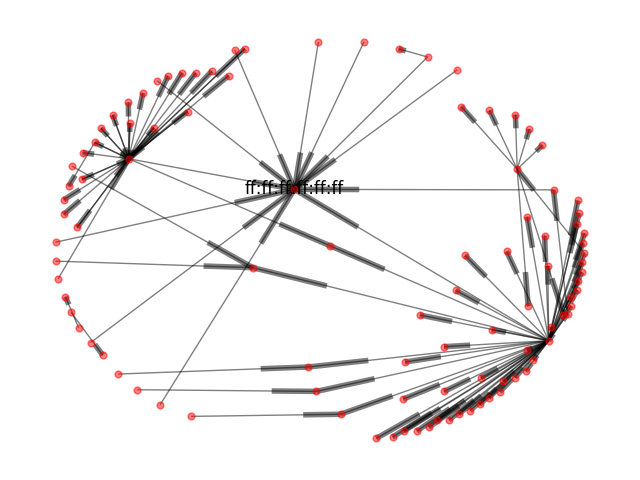
\includegraphics[scale=0.6]{../plots/labos_s2_topologia.png}
	\end{center}
\end{figure}

Como vemos, es nuevamente del tipo estrella la topologia como es esperada. Notamos una densidad
distinta de nodos en varias regiones que se pueden observar. Creemos que esto se puede deber
a la disposicion de cada laboratorio y los distintos routers o access-points que estan ubicados en la zona.
Otra observacion es que se pueden ver dos nodos arriba a la derecha de la red que no son conexos al resto del grafo.


\clearpage

\subsection{Comentarios generales}

\begin{figure}[hp!]
	\centering
	\begin{tabular}{|c|c|c|c|c|}
		\hline
		Red & Tipo & Entropía & Entropía Max & $\eta_{C}$ \\
		\hline
		Oficinas & Cableada & 2.777 & 4.858 & 0.428 \\
		\hline
		Hogareña & Wifi & 2.034 & 2.807 & 0.276 \\
		\hline
		Laboratorios & Wifi & 6.619 & 8.484 & 0.220 \\
		\hline
	\end{tabular}
	\caption[fig:tabla]{Entropía vs Max Entropía de las fuentes $S_2$ de las redes}
\end{figure}

En la figura \label{fig:tabla} se pueden ver que las redes wifi son menos compresibles ($\eta_{C}=0.276$ y $\eta_{C}=0.220$)
con respecto a la cableado ($\eta_{C}=0.428$) se puede ver en la tabla que se
reafirma nuestra hipotesis de que las redes cabledas son más compresibles que
las redes wifi.


\clearpage
\section{Conlusiones}
A modo general pudimos observar que en el caso
de la primer fuente, en todas las redes el 
símbolo destacado, o mas probable, es el unicast.
Como ya se explicó previamente esto puede deberse
a la poca cantidad de paquetes de control que suceden
en la red con respecto a la totalidad de paquetes.


Se confirmaron las hipótesis que se presentaron sobre los nodos destacados de
la fuente $S_2$. Es decir, todos estos, tenían algún propósito especial para la
red (router, impresora, access points, etc.) como lo de los niveles
de compresibilidad de los distintos tipos de redes (Cableada, Wifi).


Otra punto importante es qué se observo en todas la redes
menor cantidad de dispositivos en el gráfico de la topología
que IP's en los gráficos de probabilidad e información de la fuente $S_2$.
Esto puede deberse a que haya nodos que tenga varias IP's
o que se enviaron mensajes \textit{who-has} con IP's que no existían o dejaron
de existir en la red.

Para concluir, nos divirtió analizar las distintas redes y poder elaborar hipótesis
y comprobar resultados de los experimentos realizados. De esta forma pudimos iteriorizarnos
y comprender mejor las redes que utilizamos habitualmente.


\section{Bibliografía}
\begin{thebibliography}{9}

\bibitem{compnetworks}
  Larry L.Peterson and Bruce S. Davis,
  \emph{Computer Networks: A Systems Approach},
  Morgan Kaufmann,
  5th edition,
  2011.
\bibitem{shannon}
	Claude E. Shannon,
	\emph{A Mathematical Theory of Communication},
	The Bell System Technical Journal,
	1984,
	\url{http://math.harvard.edu/~ctm/home/text/others/shannon/entropy/entropy.pdf}
\end{thebibliography}



\end{document}
